\section{features}
A fully interactive whitted-style raytracer with run time scene loading. 
For Assignment 2, we added accelerated rendering using BVH traversal. As well as the base requirement for a BVH, we implemented option 1 of the additional options; That is, to implement an SBVH.

\subsection{BVH building}
3 BVH construction methods are available in the project -
    \begin{enumerate}
        \item Stupid: Builds a 'no-op' BVH; It will have a single root node containing all primitives. This will thus force a linear traversal of all triangles, giving almost the performance of the original assignment 1 ray tracer (although as it contains a bounding box, rays that miss the geometry entirely will be accelerated).
        \item Standard BVH: A standard BVH, constructed using the surface-area heuristic (SAH) against the longest axis of the set of primitives.
        \item SBVH: A split BVH which implements both OBJECT and SPATIAL splits against all 3 axis, "reference unsplitting" and spatial split attempt reduction.
    \end{enumerate}

\subsection{BVH traversal}
Both an ordered and unordered traversal mode is available (ordered is the default).
\subsection{Materials}
    \begin{enumerate}
    \item diffuse lighting with hard shadows
    \item reflections
    \item transparency with refraction indices
    \item specular highlights
    \item diffuse, reflective and specular values are defined by a 3-value color to match the \verb|.mtl| file format
    \item they can also be combined in arbitrary ways (i.e.\ a material can have a diffuse, reflective, transparent and specular components)
    \item triangle meshes support smoothing using barycentric interpolation of the vertex normals
    \end{enumerate}

\subsection{Run time scene loader}
    \begin{enumerate}
    \item Json scene loader
        \begin{enumerate}
        \item Triangle meshes --- loaded from file, and transformed into the world (translate, rotate, scale)
        \item Point and Spot lights
        \item camera
        \end{enumerate}
    \item \verb|.obj| file loader (using tinyojb)
    \item \verb|.mtl| material file loader (using tinyobj)
    \end{enumerate}

\subsection{Camera}
    \begin{enumerate}
    \item resizable windows
    \item zoom (mousewheel)
    \item pitch, yaw and translate
    \end{enumerate}

\subsection{Lights}
    \begin{enumerate}
    \item multi-color lighting
    \item point lights
    \item spot lights with linear falloff
    \end{enumerate}

\subsection{Vis Modes}
            FIXME: describe this ibetter
    \begin{enumerate}
    \item Default (0) - recursive Ray Trace
    \item Render Time (1)
    \item Normals (2) - 
    \item Default (3) - 
    \item Default (4) - 
    \item Default (5) -
    \item Default (6) - 
    \item Default (7) -
    \end{enumerate}

\subsection{Other}
    \begin{enumerate}
    \item multi-platform with CMake (linux, mac and windows)
    \item multi-threaded with OpenMP (got around 5x speedup on linux, which is what is expected for 4 cores with HT)
    \end{enumerate}

\section{Building}

\subsection{Building on Windows}
A visual studio solution is provided (ray.sln). This project was tested and built under Visual Studio 2015 Community. 

It should be a matter of simply loading the solution file into Visual Studio, and building. A release build is recommended as it is significantly faster.

\subsection{Building with Cmake}
The source can be built using the standard CMake envirnonment. This will work on Windows, macOS and Linux. 

For example, on unix systems this command will perform a release build -

\verb|cmake -DCMAKE_BUILD_TYPE=Release . ;| \\
\verb|make|

A similar command should work with Visual Studio, although the \verb|CMAKE_BUILD_TYPE| is not required - this is set in the Visual Studio gui.

On Windows, SDL2.dll must be available somewhere on the path or in the same dir as the binary. 

Boost is required for the test tree, but not the main system.

\section{Running}

There is a collection of test scenes, objects and materials in the data directory. To avoid fighting with relative paths, it works best to cd to this directory before running the system. For example, on windows, assuming the binary is in the Release directory under the root source tree - 

\verb|cd <source_root>\data| \\
\verb|..\Release\ray.exe teapot-plane.scene|

\section{Input Commands}
    \begin{enumerate}
    \item WASD - move around the world
    \item mouse movement - rotate camera (yaw/pitch)
    \item mouse wheel - zoom in/out (changes FOV)
    \item R - reset camera view to default (possibly set from scene file)
    \item M - Toggle barycentric smoothing
    \item P - write screenshot image
    \item C - print the current camera parameters
    \item B - change BVH construction method
    \item T - change BVH traversal method (ordered/unordered)
    \item ESC - quit
    \item 0 - view ray-traced image (default)
    \item 1 - visualise per-pixel render time (more red = more render time)
    \item 2 - visualise surface normals (useful for debugging and verifying smoothed normals)
    \item 3 - visualise BVH leaf nodes
    \item 4 - visualise triangles checked
    \item 5 - visualise BVH splits traversed
    \item 6 - visualise BVH leaves checked 
    \item 7 - visualise BVH node index
    \end{enumerate}

\section{External Packages}
The following external packages were used 
\begin{enumerate}
    \item tiny object loader --- \url{https://syoyo.github.io/tinyobjloader/}
    \item glm --- \url{https://glm.g-truc.net/0.9.8/index.html}
    \item JSON for Modern C++ --- \url{https://github.com/nlohmann/json}
    \item SDL2 --- \url{https://www.libsdl.org/download-2.0.php}
    \item boost (test tree only) --- \url{https://www.boost.org/}
    \item CMake --- \url{https://cmake.org}
\end{enumerate}

\section{Screencaps}

%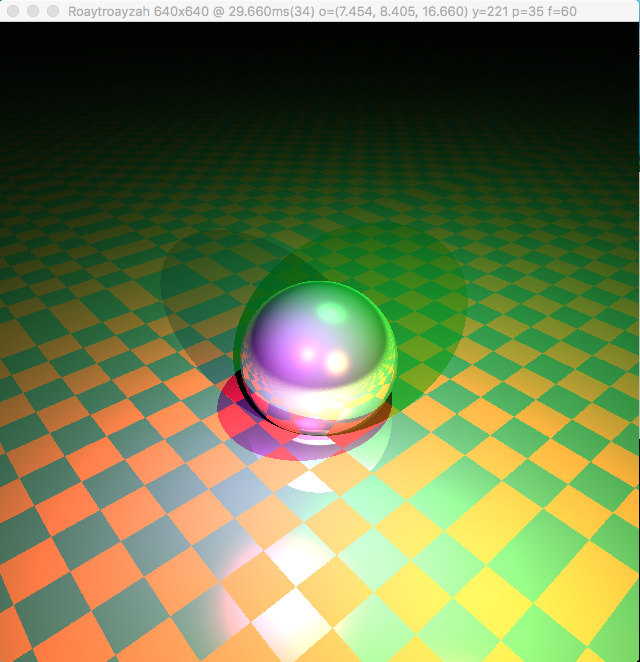
\includegraphics[width=0.5\textwidth]{img/colPointLights1sphere}
